\documentclass[11pt]{article}
\usepackage{amsmath, amssymb, amsthm}
\usepackage[retainorgcmds]{IEEEtrantools}

\usepackage[pdftex]{graphicx}
\usepackage{epstopdf}
\usepackage{tikz}
\usepackage{circuitikz}
\usetikzlibrary{intersections}

\usepackage{fancyhdr}

%Listings stuff
\usepackage{listings}
\usepackage{lstautogobble}
\usepackage{color}

\definecolor{gray}{rgb}{0.5,0.5,0.5}
\lstset{
basicstyle={\small\ttfamily},
tabsize=3,
numbers=left,
numbersep=5pt,
numberstyle=\tiny\color{gray},
stepnumber=2,
breaklines=true,
boxpos=t
}

%Format stuff
\pagestyle{fancy}
\headheight 35pt

%Header info
\chead{\Large \textbf{Closest Pair}}
\lhead{}
\rhead{}

\begin{document}
\section{Algorithm}
	Given a list of 2D points $P$, find the pair with the minimum Euclidean distance between them. We assume that the input is presorted by both $x$ and $y$ coordinates, so $P = (P_x, P_y)$. Divide and conquer by splitting the input points in half x-wise, and combining results.
	
	\begin{lstlisting}[autogobble=true,mathescape]
		closestPair(P = (Px, Py)):
			if |P| <= 3: brute force
			else:
				l = x-coordinate of median of Px
				PL, PR = halves of Px split along l
				dL = closestPair(PL)
				dR = closestPair(PR)
				d = min(dL, dR)
				
				Sy = {p if |p.x - l| <= d for p in Py}
				d' = stripClosest(Sy)
				
				return min(d, d')
				
		stripClosest(Sy):
			d' = $\infty$
			for i in [1, |Sy|]:
				for j in [i + 1, min(|Sy|, i + 7)]:
					if ||Sy[i], Sy[j]|| <= d':
						d' = ||Sy[i], Sy[j]||
						
			return d'
	\end{lstlisting}
	
	While we can get the shortest distance between any two points in each half of the divided point set through recursion, it's also possible that the true shortest distance is between two points that straddle the divide at $l$, which is what the \verb|stripClosest| function checks for.
	
\section{Runtime}
	Initial sorting by x- and y-coordinate of the input set is $\Theta(n\log n)$. Recursion depth is $\Theta(\log n)$, with $\Theta(n)$ work done on each call, so the total runtime is $\Theta(n\log n)$. Formally speaking, the recurrance is given by
	\begin{equation}
		T(n) = 2T\left( \frac{n}{2} \right) + 7n + O(1)
	\end{equation}
	
\section{Proof}
	Consider the following situation, where we have the shortest distances between pairs on just the left and right sides, and took the minimum as $\delta$:
	
	\begin{figure}[htb]
		\centering
		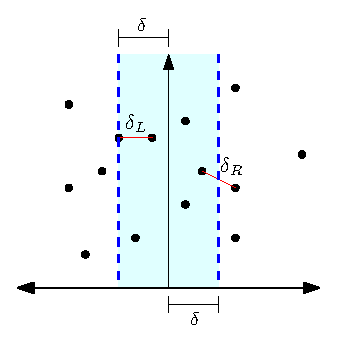
\includegraphics{closest-pair.eps}
	\end{figure}
	
	If $\exists (p, q) \in P \mid ||p, q|| < \delta$ and $p$ and $q$ are on different sides, then the x-coordinate of both points must be within $\delta$ of $l$. Let $S_y$ be the set of points in $P$ sorted by y-coordinate that lie within this strip.
	
	\subparagraph{Claim} Given $s_i, s_j \in S_y$, if $||s_i, s_j|| \leq \delta$, then $|j - i| \leq 7$.
	
	\subparagraph{Proof} Assume $||s_i, s_j|| \leq \delta$. The two points then must be inside the $\delta$-strip of $l$ x-wise, and their y-coordinates can differ by at most $\delta$.  This forms a $\delta \times 2\delta$ rectangular area that this pair can lie within.
	
	\begin{figure}[htb]
		\centering
		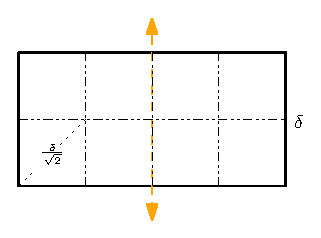
\includegraphics{closest-pair-square.eps}
	\end{figure}
	
	Now split this rectangle into 8 equal squares of $\delta/2 \times \delta/2$ each. The diagonal length of each square is $\delta/\sqrt{2}$, which is less than $\delta$. Given that on each half, the closest pair has distance equal to or greater than $\delta$, this means that only one point can be in each square. Since the number of points in the rectangle is therefore upper-bounded by 8, $|j - i| \leq 7$.

%	\begin{center}
%	\begin{tikzpicture}
%		[scale=3,line cap=round,
%		%Styles
%		axes/.style=,
%		important line/.style={very thick},
%		information text/.style={rounded corners,fill=red!10,inner sep=1ex},
%		dot/.style={circle,inner sep=1pt,fill,label={#1},name=#1}			
%		]
%		
%		%Colors
%		\colorlet{anglecolor}{green!50!black}	%angle arcs/lines
%		
%		%The graphic
%	\end{tikzpicture}
%	\end{center}

%	\begin{figure}[htb]
%		\centering
%		\includegraphics[width=0.8\textwidth]{filename.eps}
%		\caption{Caption.}
%		\label{fig:figure}
%	\end{figure}

%		\def\enotesize{\normalsize}
%		\theendnotes
\end{document}